\documentclass[]{standalone}
\usepackage{color}
\usepackage{bm}
\usepackage{amssymb}
\usepackage{tikz}
\usetikzlibrary{shapes,arrows,arrows.meta,fit,positioning}
\usetikzlibrary{chains,quotes}

\newcommand{\defaultwidth}{2cm}
\newcommand{\tseparation}{0.7cm}
\tikzset{
    auto, node distance = 2cm,
    stage/.style = { draw, very thick, rectangle, align=center,
        node distance = 1cm,
        text width = \defaultwidth, 
        font=\bfseries,
        rounded corners=2mm, 
        minimum width = \defaultwidth
    },
    bstage/.style = { very thick, rectangle, align=center,
        node distance = 1cm,
        text width = \defaultwidth, 
        font=\bfseries, color=white,
        rounded corners=2mm, 
        minimum width = \defaultwidth
    },
    op/.style = { align=center,
        node distance = 0.25cm,
        font=\bfseries
    },
    notes/.style = { draw, very thin, rectangle, dashed, align=left,
        node distance = 1.5cm,
        text width = \defaultwidth + 1.5cm, 
        font=\footnotesize,
        minimum width = \defaultwidth + 1.5cm
    },
    arrow_text/.style = { align=left,
        pos = 0.5,
        text width = \defaultwidth, 
        font = \footnotesize,
        minimum width = \defaultwidth
    },
    point/.style = { draw, circle, fill,
        inner sep = 0.06cm,
        node contents={}
    },
    aline/.style = { very thick, minimum width = 10cm },
    arrow/.style = { dashed, ->, >=stealth }
}

\begin{document}
    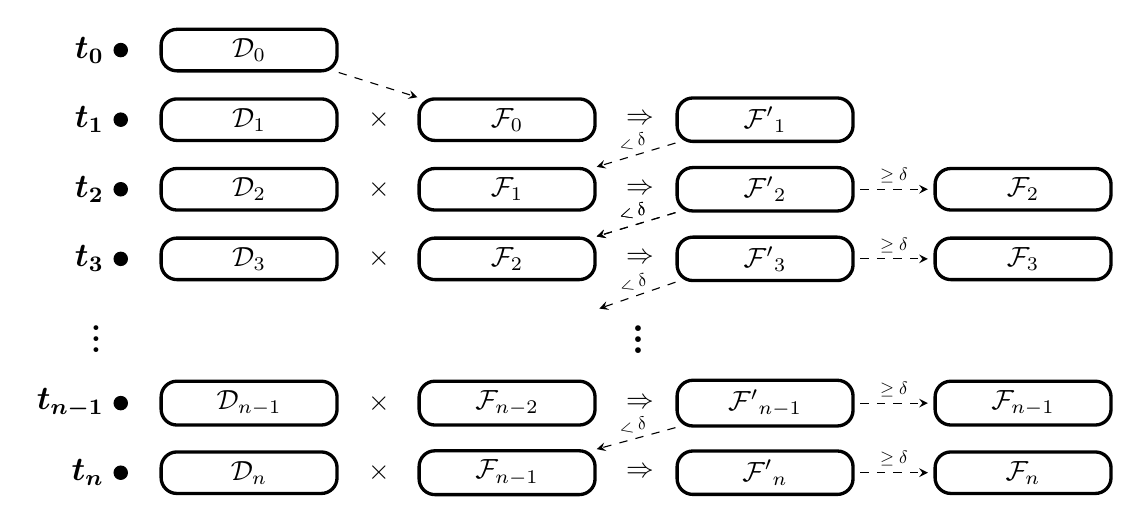
\begin{tikzpicture}
        \node (t0) at (0,0) [label=left:{\large \bm{$t_0$}}, point];
        \node (t1) [below=\tseparation of t0] [label=left:{\large \bm{$t_1$}}, point];
        \node (t2) [below=\tseparation of t1] [label=left:{\large \bm{$t_2$}}, point];
        \node (t3) [below=\tseparation of t2] [label=left:{\large \bm{$t_3$}}, point];
        \node (t4) [below=\tseparation of t3] [label=left:{\large \bm{$\vdots$}}]{};
        \node (t5) [below=\tseparation of t4] [label=left:{\large \bm{$t_{n-1}$}}, point];
        \node (t6) [below=\tseparation of t5] [label=left:{\large \bm{$t_{n}$}}, point];

        % t0 branch...
        \node[stage, node distance=0.4cm] (t01) [right = of t0]    {$\mathcal{D}_{0}$}; 
        % t1 branch...
        \node[stage, node distance=0.4cm] (t11) [right = of t1]    {$\mathcal{D}_{1}$}; 
        \node[stage] (t12) [right = of t11]  {$\mathcal{F}_{0}$}; 
        \path (t11) node[op,right=of t11]{$\times$} (t12);
        \node[stage] (t13) [right = of t12]  {$\mathcal{F'}_{1}$}; 
        \path (t12) node[op,right=of t12]{$\Rightarrow$} (t13);
        % t2 branch...
        \node[stage, node distance=0.4cm] (t21) [right = of t2]    {$\mathcal{D}_{2}$}; 
        \node[stage] (t22) [right = of t21]  {$\mathcal{F}_{1}$}; 
        \path (t21) node[op,right=of t21]{$\times$} (t22);
        \node[stage] (t23) [right = of t22]  {$\mathcal{F'}_{2}$}; 
        \path (t22) node[op,right=of t22]{$\Rightarrow$} (t23);
        \node[stage] (t24) [right = of t23]  {$\mathcal{F}_{2}$}; 
        % t3 branch...
        \node[stage, node distance=0.4cm] (t31) [right = of t3]    {$\mathcal{D}_{3}$}; 
        \node[stage] (t32) [right = of t31]  {$\mathcal{F}_{2}$}; 
        \path (t31) node[op,right=of t31]{$\times$} (t32);
        \node[stage] (t33) [right = of t32]  {$\mathcal{F'}_{3}$}; 
        \path (t32) node[op,right=of t32]{$\Rightarrow$} (t33);
        \node[stage] (t34) [right = of t33]  {$\mathcal{F}_{3}$}; 
        % t4 branch...
        \node[bstage, node distance=0.4cm] (t41) [right = of t4]    {}; 
        \node[bstage] (t42) [right = of t41]  {$\mathcal{F}_{3}$}; 
       
        %\node[node distance=1.5cm] (t41) [right = of t4]    {}; 
        %\node[text width = \defaultwidth, minimum width = \defaultwidth, align=right] (t42) [right = of t41]  {\bm{$\vdots$}}; 
        %\node[] (t43) [right = of t42]  {}; 
        %\node[] (t44) [right = of t43]  {}; 
        % t5 branch...
        \node[stage, node distance=0.4cm] (t51) [right = of t5]    {$\mathcal{D}_{n-1}$}; 
        \node[stage] (t52) [right = of t51]  {$\mathcal{F}_{n-2}$}; 
        \path (t51) node[op,right=of t51]{$\times$} (t52);
        \node[stage] (t53) [right = of t52]  {$\mathcal{F'}_{n-1}$}; 
        \path (t52) node[op,right=of t52]{$\Rightarrow$} (t53);
        \node[stage] (t54) [right = of t53]  {$\mathcal{F}_{n-1}$}; 
        % t6 branch...
        \node[stage, node distance=0.4cm] (t61) [right = of t6]    {$\mathcal{D}_{n}$}; 
        \node[stage] (t62) [right = of t61]  {$\mathcal{F}_{n-1}$}; 
        \path (t61) node[op,right=of t61]{$\times$} (t62);
        \node[stage] (t63) [right = of t62]  {$\mathcal{F'}_{n}$}; 
        \path (t62) node[op,right=of t62]{$\Rightarrow$} (t63);
        \node[stage] (t64) [right = of t63]  {$\mathcal{F}_{n}$}; 

        \node (tv) [right=6.65cm of t4] [label=left:{\Large \bm{$\vdots$}}]{};
        
        % arrows...
        \draw[arrow] (t01.south east) -- (t12.north west);
        \draw[arrow] (t13.south west) -- node[above,sloped,scale=0.65] {$<\delta$} (t22.north east);
        \draw[arrow] (t23.south west) -- node[above,sloped,scale=0.65] {$<\delta$} (t32.north east);
        \draw[arrow] (t23.south west) -- node[above,sloped,scale=0.65] {$<\delta$} (t32.north east);
        \draw[arrow] (t33.south west) -- node[above,sloped,scale=0.65] {$<\delta$} (t42.north east);
        \draw[arrow] (t53.south west) -- node[above,sloped,scale=0.65] {$<\delta$} (t62.north east);
        \draw[arrow, shorten >= 2pt, shorten <= 2pt] (t23.east) -- node[above,sloped,scale=0.65] {$\geq \delta$} (t24.west);
        \draw[arrow, shorten >= 2pt, shorten <= 2pt] (t33.east) -- node[above,sloped,scale=0.65] {$\geq \delta$} (t34.west);
        \draw[arrow, shorten >= 2pt, shorten <= 2pt] (t53.east) -- node[above,sloped,scale=0.65] {$\geq \delta$} (t54.west);
        \draw[arrow, shorten >= 2pt, shorten <= 2pt] (t63.east) -- node[above,sloped,scale=0.65] {$\geq \delta$} (t64.west);
        
    \end{tikzpicture}
\end{document}
